\documentclass[aspectratio=169,mathserif]{beamer}
%\documentclass[aspectratio=169,mathserif,handout]{beamer}

\usepackage{graphicx} % Allows including images
\graphicspath{{./img/}}

\usepackage{epstopdf}
\epstopdfsetup{outdir=./img/}

\usepackage[utf8]{inputenc}
%Load useful packages
\usepackage{booktabs} % Allows the use of \toprule, \midrule and \bottomrule in tables
\usepackage{subcaption}
\usepackage{subfiles}
\usepackage{url}
\usepackage{amssymb}
%
\usepackage{multirow}
%
% align enum description
% \usepackage{enumitem}
% refs
\usepackage[style=authoryear,natbib=true]{biblatex}
\bibliography{references.bib}
%
\usepackage{tikz}
\usepackage{tikz-cd}
\usepackage{tikzscale}
\usetikzlibrary{calc,matrix,chains,positioning,decorations.pathreplacing,decorations.text,arrows,cd}

% overlays
\tikzset{
invisible/.style={opacity=0},
visible on/.style={alt={#1{}{invisible}}},
alt/.code args={<#1>#2#3}{%
\alt<#1>{\pgfkeysalso{#2}}{\pgfkeysalso{#3}} % \pgfkeysalso doesn't change the path
},
}

% neural nets
\tikzset{%
  every neuron/.style={
circle,
draw,
%minimum size=1cm
  },
  neuron missing/.style={
draw=none, 
scale=1,
text height=0.333cm,
execute at begin node=\color{black}$\vdots$
  },
}

% infrastructure
\tikzset{
vertex/.style = {
circle,
fill= black,
outer sep = 2pt,
inner sep = 1pt,
}
}




%Information to be included in the title page:
\title{Deep Learning}
\subtitle{Perceptron}

\author{Tiago Vieira}
\institute{Institute of Computing\\Universidade Federal de Alagoas}
\date{\today}
%Logo in every slide
\logo{%
  \makebox[0.98\paperwidth]{

\includegraphics[width=0.5cm,keepaspectratio]{logos/ufal_logo.png}%
\hfill%
\includegraphics[height=1cm,keepaspectratio]{logos/edge_logo.png}%

\includegraphics[height=0.8cm,keepaspectratio]{logos/ic_logo.png}%
  }
}
%Contents before every section's starting slide
\AtBeginSubsection[]
{
  \begin{frame}
\frametitle{Summary}
\scriptsize
\tableofcontents[currentsection,currentsubsection]
  \end{frame}


}
% shape, colour of item, nested item bullets in itemize only
% \setbeamertemplate{itemize item}[square] \setbeamercolor{itemize item}{bg=blue}
% \setbeamertemplate{itemize subitem}[circle] \setbeamercolor{itemize subitem}{fg=green}
% \setbeamertemplate{itemize subsubitem}[triangle] \setbeamercolor{itemize subsubitem}{fg=red}
% font size of nested and nested-within-nested bulltes in both itemize and enumerate
% options are \tiny, \small, \scriptsize, \normalsize, \footnotesize, \large, \Large, \LARGE, \huge and \Huge
\setbeamerfont{itemize/enumerate subbody}{size=\scriptsize} 
\setbeamerfont{itemize/enumerate subsubbody}{size=\scriptsize}
% figure numbers
% \setbeamertemplate{caption}[numbered]
% blocks style
\setbeamertemplate{blocks}[rounded][shadow=true]


% Hide nav control
\usenavigationsymbolstemplate{}
% add numbering
\addtobeamertemplate{navigation symbols}{}{%
\usebeamerfont{footline}%
\usebeamercolor[fg]{footline}%
\hspace{1em}%
\insertframenumber/\inserttotalframenumber
}

% Footnote without number
\newcommand\blfootnote[1]{%
\begingroup
\renewcommand\thefootnote{}\footnote{#1}%
\addtocounter{footnote}{-1}%
\endgroup
}

% items symbols
\setbeamertemplate{itemize subitem}{-}
\setbeamertemplate{itemize subsubitem}{-}

%%setting up some useful slide creation commands
%split slide
% \newenvironment{splitframe}[5]
% %[1] ==> 1 parameter passed through {}
% %[2] ==> 2 parameters passed through {}{}
% %[4] ==> 4 parameters passed through {}{}{}{}
% {
% \begin{frame}{#3}
% \begin{columns}
% \column{#1\linewidth}
% \centering
% #4
% \column{#2\linewidth}
% \centering
% #5
% \end{columns}
% \centering
% \vspace{\baselineskip} % adds one line space
% }
% %Inside the first pair of braces (ABOVE) is set what your new environment will do before the text within, then inside the second pair of braces (BELOW) declare what your new environment will do after the text. Note second pair can be empty braces too.
% {
% \end{frame}


% }

\begin{document}

\frame{\titlepage}

%\begin{frame}
%\frametitle{Summary}
%{\tableofcontents}
%\end{frame}

\begin{frame}{Motivation}
\begin{figure}[!]
\centering
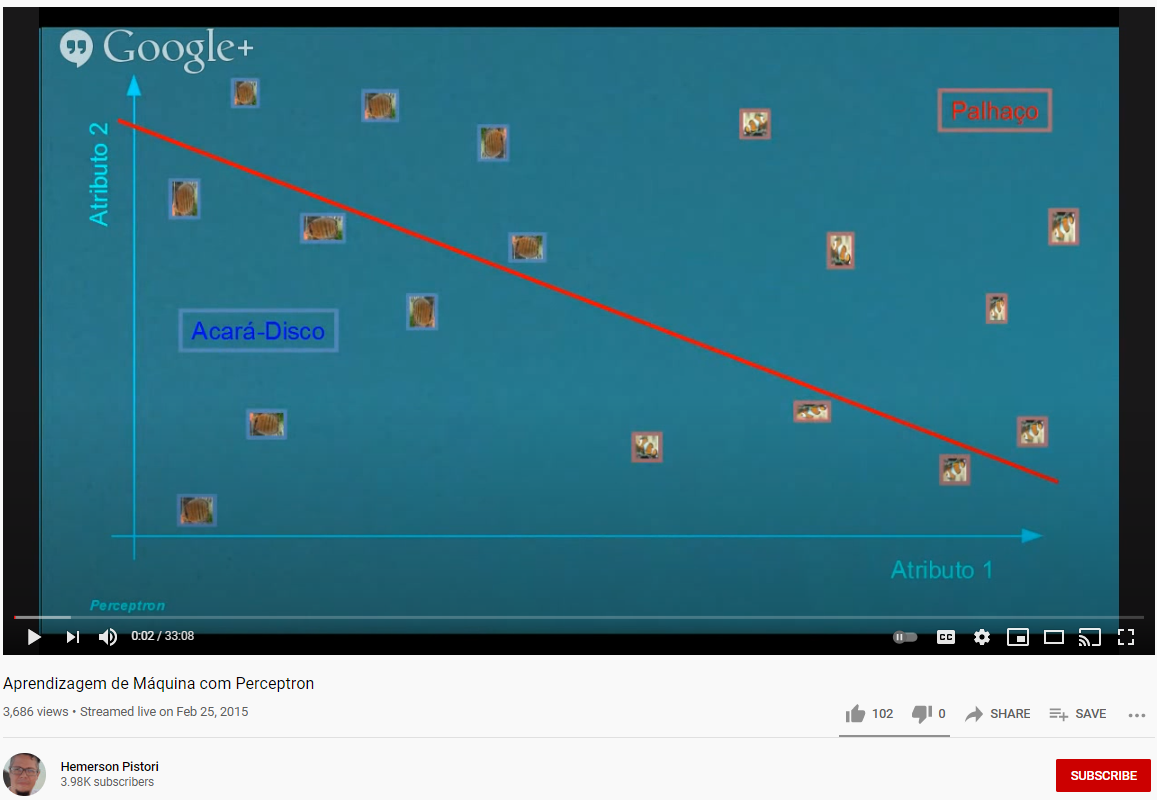
\includegraphics[width=.7\textwidth]{ml-com-perceptron.png}
\end{figure}
\footnote{\href{https://www.youtube.com/watch?v=-C07ansuc-8}{Aprendizagem de máquina com o Perceptron.}}
\end{frame}


\begin{frame}{Motivation}
\begin{figure}[!]
\centering
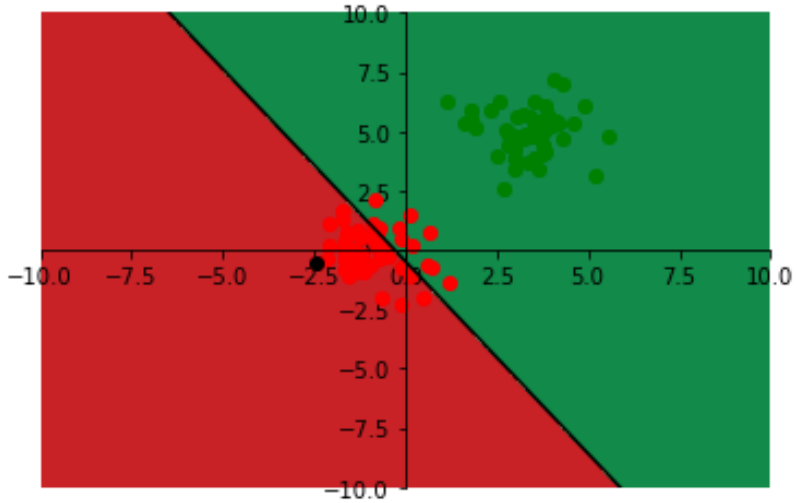
\includegraphics[width=.7\textwidth]{perceptrong}
\end{figure}
\footnote{\href{https://github.com/tfvieira/deep-learning/blob/main/src/simple_perceptron/simple_perceptron.py}{Simple perceptron example using NumPy}}
\end{frame}




\begin{frame}
\frametitle{Binary Classification and Linear Regression Problems}
\begin{itemize}
\item In the binary classification problem, each training pair $(\overline{X}, y)$ contains feature variables $\overline{X}=(x_1, \ldots x_d)$, and  label
$y$  drawn from $\{ -1, +1 \}$.
\begin{itemize}
\item Example: Feature variables might be frequencies of words in an
email, and the class variable might be an indicator of spam.
\item Given labeled emails,  recognize incoming spam.
\end{itemize}
\item In linear regression, the {\em dependent} variable $y$ is real-valued.
\begin{itemize}
\item Feature variables are frequencies of words in a Web page,
and the  dependent variable is a prediction of the number of
accesses in a fixed period.
\end{itemize}
\item Perceptron is designed for the binary setting.
\end{itemize}
\end{frame}



\begin{frame}
\frametitle{The Perceptron: Earliest Historical Architecture}
\begin{center}
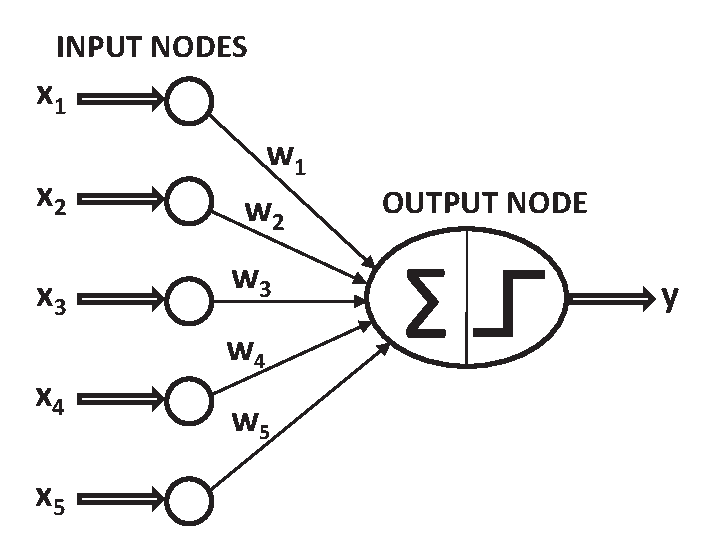
\includegraphics[scale=0.4]{neurala.eps}
\end{center}
\begin{itemize}
\item The  $d$ nodes in the input layer only transmit the $d$
features $\overline{X}=[x_1 \ldots x_d]$ without performing any
computation.
\item  Output
node   multiplies input with  weights $\overline{W}=[w_1 \ldots
w_d]$ on incoming edges, aggregates them, and applies  {\em sign
activation}:
\begin{equation*}
\hat{y}= \mbox{sign}\{ \overline{W}\cdot \overline{X} \} =
\mbox{sign}\{ \sum_{j=1}^d w_j x_j \} \label{1nobias}
\end{equation*}
\end{itemize}
\end{frame}



\begin{frame}
\frametitle{What is the Perceptron Doing?}
\begin{itemize}
\item Tries to find a {\em linear separator} $\overline{W}\cdot \overline{X}=0$ between the two
classes. \item  Ideally, all positive instances ($y=1$) should be on
the side of the separator satisfying $\overline{W} \cdot
\overline{X}>0$.
 \item  All negative  instances ($y=-1$) should be on the
side of the separator satisfying $\overline{W} \cdot
\overline{X}<0$.
\end{itemize}
\end{frame}



\begin{frame}
\frametitle{Bias Neurons}
%%%%%%%%%%%%%%%%%%%%%%%%%%%%%%%%%%%%%%%%%%%%%%%%%%%%%%%%%%%%%%%%%%%%%%%%%
\begin{center}
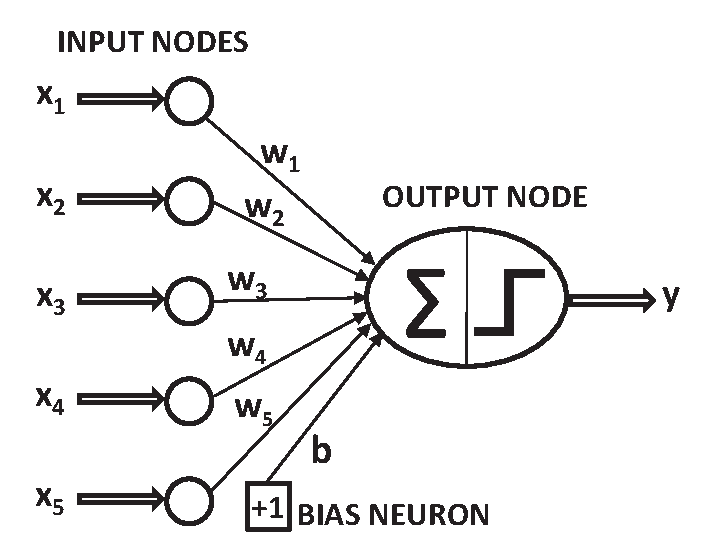
\includegraphics[scale=0.4]{neuralbiasa.eps}
\end{center}
\begin{itemize}
\item  In many settings (e.g., skewed class distribution) we need an
invariant part of the prediction with bias variable $b$:
\begin{equation*}
\hat{y}= \mbox{sign}\{ \overline{W}\cdot \overline{X} +b \} =
\mbox{sign}\{ \sum_{j=1}^d w_j x_j  + b  \} = \mbox{sign}\{
\sum_{j=1}^{d+1} w_j x_j    \}
\end{equation*}
\item On setting $w_{d+1}=b$ and $x_{d+1}$ as the input from the
bias neuron, it makes little difference to learning procedures
$\Rightarrow$ Often implicit in architectural diagrams
\end{itemize}
\end{frame}


\begin{frame}
\frametitle{Training a Perceptron}
\begin{itemize}
\item Go through the input-output pairs $(\overline{X}, y)$ one by one and make
updates, if predicted value $\hat{y}$ is different from observed
value $y$ $\Rightarrow$ Biological readjustment of synaptic weights.
\begin{eqnarray*}
& \overline{W}  \Leftarrow  \overline{W} +
\alpha \underbrace{(y - \hat{y})}_{\mbox{Error}} \overline{X}\\
& \overline{W}  \Leftarrow  \overline{W} + (2 \alpha)  y
\overline{X} \ \mbox{[For misclassified instances $y -\hat{y}= 2y$]}
\end{eqnarray*}
\item Parameter $\alpha$ is the learning rate $\Rightarrow$ Turns
out to be irrelevant in the special case of the perceptron
\item One cycle through the entire training data set is referred to
as an {\em epoch} $\Rightarrow$ Multiple epochs required
\item How did we derive these updates?
\end{itemize}
\end{frame}




\begin{frame}
\frametitle{What Objective Function is the Perceptron Optimizing?}
\begin{itemize}
\item At the time, the perceptron was proposed, the notion of loss
function was not popular $\Rightarrow$ Updates were heuristic

\item  Perceptron optimizes the perceptron criterion for $i$th training instance:
\begin{equation*}
 L_i= \mbox{max} \{ -y_i (\overline{W}\cdot \overline{X_i}), 0 \}
\end{equation*}
\begin{itemize}
\item Loss function tells us how far we are from a desired solution
$\Rightarrow$ Perceptron criterion is  0 when $\overline{W} \cdot
\overline{X_i}$ has same sign as $y_i$.
\end{itemize}
\item  Perceptron updates use  {\em stochastic gradient descent} to optimize the loss function and reach
the desired outcome.
\begin{itemize}
\item Updates are equivalent to $\overline{W} \Leftarrow  \overline{W}
- \alpha \left( \frac{\partial L_i}{\partial w_1} \ldots
\frac{\partial L_i}{\partial w_d} \right)$ \end{itemize}
\end{itemize}
\end{frame}


%\begin{frame}
%\frametitle{Perceptron vs Linear SVMs}
%\begin{itemize}
%\item Perceptron criterion
% is a shifted version of hinge-loss in SVM:
%\begin{equation*}
% L^{svm}_i = \mbox{max} \{ 1-y_i (\overline{W}\cdot \overline{X_i}), 0 \}
%\end{equation*}
%\begin{itemize}
%\item  The pre-condition for updates in perceptron and SVMs is different: \end{itemize}
%\begin{itemize}
%\item In a perceptron, we update when a misclassification occurs: $-y_i (\overline{W}\cdot
%\overline{X_i})>0$
%\item In a linear SVM, we update when a misclassification occurs or a classification is ``barely correct'': $1-y_i (\overline{W}\cdot
%\overline{X_i})>0$
%\end{itemize}
%\item Otherwise, {\em primal} updates of linear SVM are {\em identical} to perceptron: $$\overline{W}  \Leftarrow  \overline{W} +  \alpha  y
%\overline{X}$$
%\end{itemize}
%\end{frame}
%
%
%
%\begin{frame}
%\frametitle{Perceptron vs Linear SVMs}
%\begin{center}
%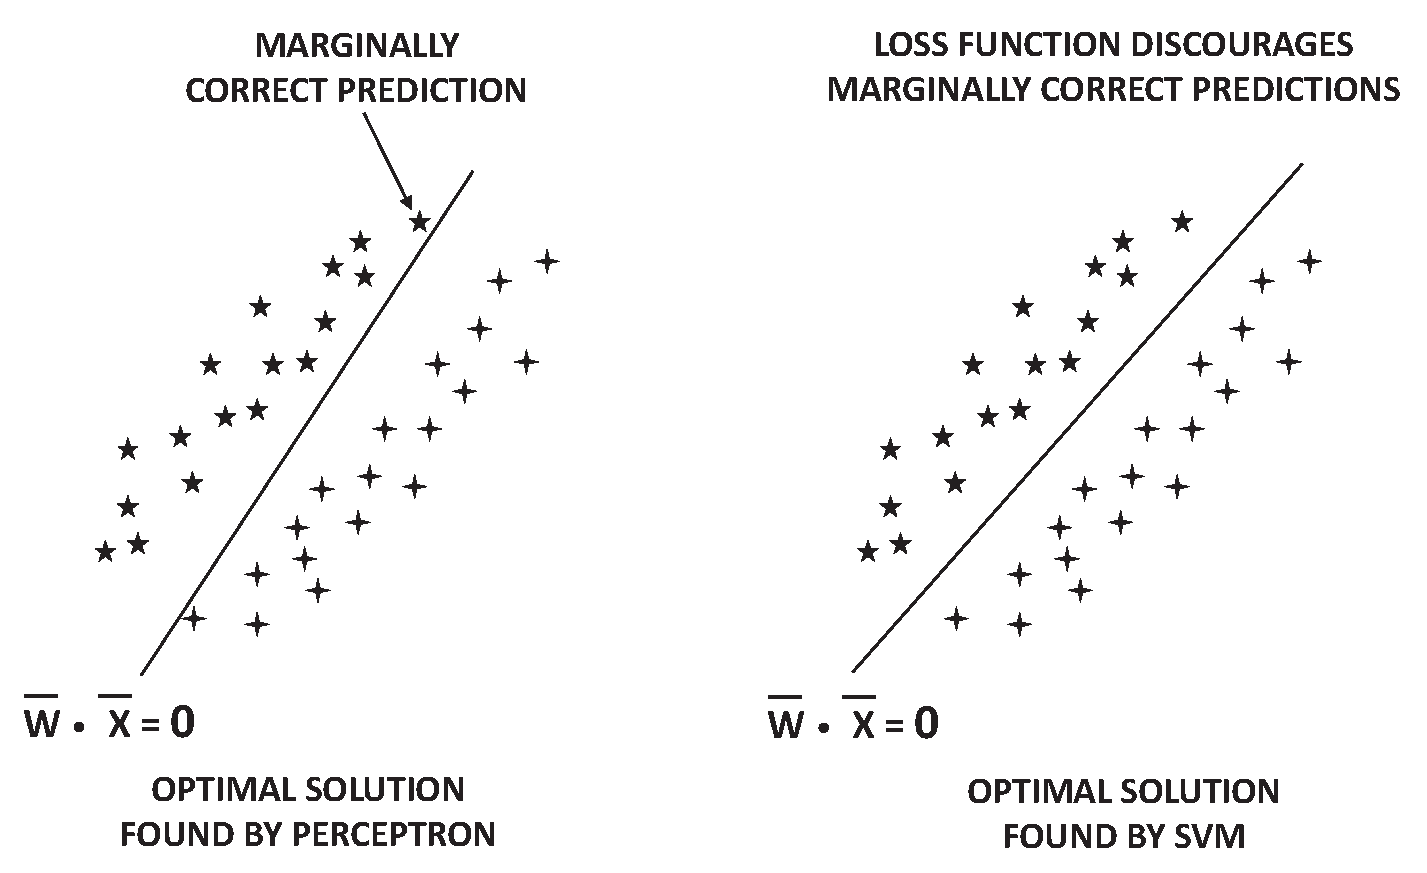
\includegraphics[scale=0.35]{compare.eps}
%\end{center}
%\begin{itemize}
%\item The more rigorous condition for the update in a linear SVM
%ensures that points near the decision boundary {\em generalize}
%better to the test data.
%\end{itemize}
%\end{frame}


\begin{frame}
\frametitle{Where does the Perceptron Fail?}
\begin{center}
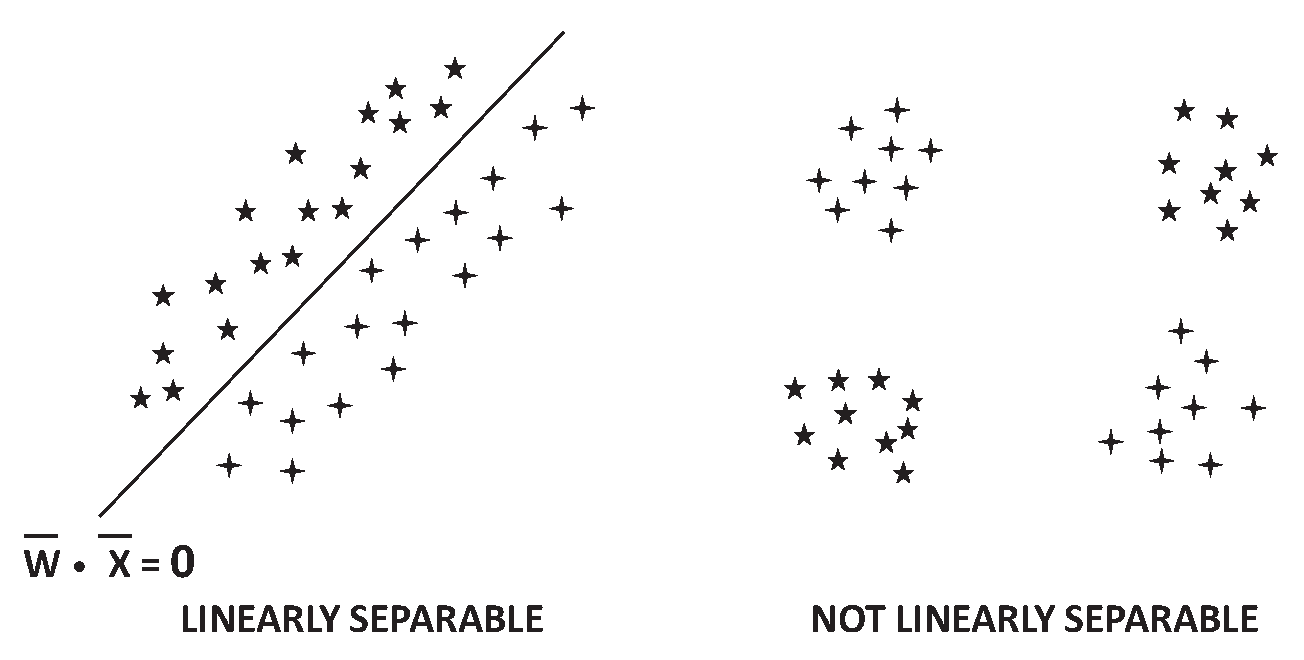
\includegraphics[scale=0.4]{separable.eps}
\end{center}
\begin{itemize}
\item The perceptron fails at similar problems as a linear SVM
\begin{itemize}
\item {\bf Classical solution:} Feature engineering with
Radial Basis Function network $\Rightarrow$ Similar to kernel SVM
and good for noisy data
\item {\bf Deep learning solution:} Multilayer networks with
nonlinear activations $\Rightarrow$ Good for data with a lot of
structure
\end{itemize}
\end{itemize}
\end{frame}




\begin{frame}
\frametitle{Historical Origins}
\begin{itemize}
\item The first  model of a computational unit was the {\em
perceptron} (1958).
\begin{itemize}
\item Was roughly inspired by the biological model of a neuron.
\item Was implemented using a large piece of hardware.
\item Generated great excitement but failed to live up to inflated expectations.
\end{itemize}
\item Was not any more powerful than a simple linear model that can
be implemented in a  few lines of code today.
\end{itemize}
\end{frame}



%\begin{frame}
%\frametitle{The Perceptron [Image Courtesy: Smithsonian Institute]}
%\begin{center}
%\includegraphics[scale=1.2]{mark1.eps}
%\end{center}
%\end{frame}


%\begin{frame}{References}
%\footnotesize{
%\bibitem[Gonzalez2012]{p1} Aggarwal, C. C. (2018)
%\newblock Neural Networks and Deep Learning (1st ed.).
%\newblock \emph{Springer International Publishing} 1$^{th}$ Ed..
%%
%%\bibitem[Gonzalez2012]{p1} Gonzalez, Rafael C.; Woods, Richard E. (2018)
%%\newblock Digital Image Processing
%%\newblock \emph{Pearson} 4$^{th}$ Ed..
%%
%%\bibitem[Gonzalez2009]{p1} Gonzalez, Rafael C.; Woods, Richard E. (2009)
%%\newblock Digital Image Processing Using Matlab
%%\newblock \emph{Pearson} 2$^{nd}$ Ed..
%%\end{thebibliography}
%%}
%\end{frame}


\end{document}
